\section{Experiment}
This section presents an empirical study on MOS-RMBench to investigate the performance of different paradigms. We first present the overall evaluation results, then perform an error analysis across samples with varying MOS gaps, and finally explore a MOS-aware GRM designed to address the limitations revealed by this analysis.


\begin{table}[htbp]
\centering
% \setlength{\abovecaptionskip}{-0.1cm} % 调整间距
\setlength{\belowcaptionskip}{0.2cm}
\caption{Evaluation results of models from different paradigms on MOS-RMBench. The best results are shown in \textbf{bold} and the second best is with \uline{underline}.}

\renewcommand{\arraystretch}{1.1} % 行距

\label{tab:main-results}
\resizebox{\textwidth}{!}{
\begin{tabular}{l|cccccc|c}
\toprule
\textbf{Model} & \textbf{BVCC} & \textbf{NISQA} & \textbf{SingMOS} & \textbf{SOMOS} & \textbf{TMHINT-QI} & \textbf{VMC'23} & \textbf{Overall} \\
\midrule
\rowcolor[rgb]{ .792,  .87,  .949} \multicolumn{8}{c}{\textit{MOS prediction model}} \\
UTMOS & \textbf{86.70} & 73.17 & 63.80 & 65.00 & 68.10 & 60.83 & 68.18 \\
\midrule
\rowcolor[rgb]{ .792,  .87,  .949} \multicolumn{8}{c}{\textit{LLM-as-a-judge}} \\
Gemini-2.5-Pro     & 63.90 & 81.96 & 58.50 & 64.10 & 73.20 & 65.57 & 69.26 \\
Qwen2.5-Omni-7B    & 54.00 & 63.97 & 57.70 & 56.30 & 69.90 & 58.43 & 60.23 \\
\midrule
\rowcolor[rgb]{ .792,  .87,  .949} \multicolumn{8}{c}{\textit{Scalar reward models}} \\
Classic + BT Loss  & \uline{85.70} & \textbf{83.93} & 74.80 & \textbf{76.80} & \textbf{81.10} & \textbf{77.73} & \textbf{80.04} \\
Classic + MSE Loss & 82.80 & 79.33 & 69.80 & 74.30 & 79.40 & 72.23 & 75.83 \\
\midrule
\rowcolor[rgb]{ .792,  .87,  .949} \multicolumn{8}{c}{\textit{Semi-scalar reward models}} \\
Cloud + BT Loss    & 85.50 & 81.07 & \textbf{78.20} & \uline{75.30} & \uline{80.60} & \uline{75.70} & \uline{78.82} \\
Cloud + MSE Loss   & 84.50 & 77.81 & 76.10 & 75.20 & 80.50 & 73.67 & 77.01 \\

\midrule
\rowcolor[rgb]{ .792,  .87,  .949} \multicolumn{8}{c}{\textit{Generative reward models}} \\
GRM + SFT          & 80.60 & 79.60 & 75.10 & 70.00 & 77.90 & 69.23 & 74.63 \\
GRM + GRPO         & 82.50 & 80.31 & 76.40 & 74.60 & 78.10 & 73.13 & 76.94 \\
GRM + DAPO         & 82.60 & \uline{82.05} & \uline{77.50} & 74.40 & 79.30 & 73.13 & 77.60 \\
\bottomrule
\end{tabular}
}
\vskip -0.05in
\end{table}



% \begin{table}[htbp]
% \centering
% % \setlength{\abovecaptionskip}{-0.1cm} % 调整间距
% \setlength{\belowcaptionskip}{0.2cm}
% \caption{Evaluation results of models from different paradigms on MOS-RMBench. The best results are shown in \textbf{bold} and the second best is with \uline{underline}.}

% \renewcommand{\arraystretch}{1.1} % 行距

% \label{tab:main-results}
% \resizebox{\textwidth}{!}{
% \begin{tabular}{lccccccc}
% \toprule
% \textbf{Model} & \textbf{BVCC} & \textbf{NISQA} & \textbf{SingMOS} & \textbf{SOMOS} & \textbf{TMHINT-QI} & \textbf{VMC'23} & \textbf{Overall} \\
% \midrule
% \multicolumn{8}{c}{\textit{MOS prediction model}} \\
% UTMOS & \textbf{86.70} & 73.17 & 63.80 & 65.00 & 68.10 & 60.83 & 68.18 \\
% \midrule
% \multicolumn{8}{c}{\textit{LLM-as-a-judge}} \\
% Gemini-2.5-Pro     & 63.90 & 81.96 & 58.50 & 64.10 & 73.20 & 65.57 & 69.26 \\
% Qwen2.5-Omni-7B    & 54.00 & 63.97 & 57.70 & 56.30 & 69.90 & 58.43 & 60.23 \\
% \midrule
% \multicolumn{8}{c}{\textit{Scalar reward models}} \\
% Classic + BT Loss  & \uline{85.70} & \textbf{83.93} & 74.80 & \textbf{76.80} & \textbf{81.10} & \textbf{77.73} & \textbf{80.04} \\
% Classic + MSE Loss & 82.80 & 79.33 & 69.80 & 74.30 & 79.40 & 72.23 & 75.83 \\
% \midrule
% \multicolumn{8}{c}{\textit{Semi-scalar reward models}} \\
% Cloud + BT Loss    & 85.50 & 81.07 & \textbf{78.20} & \uline{75.30} & \uline{80.60} & \uline{75.70} & \uline{78.82} \\
% Cloud + MSE Loss   & 84.50 & 77.81 & 76.10 & 75.20 & 80.50 & 73.67 & 77.01 \\

% \midrule
% \multicolumn{8}{c}{\textit{Generative reward models}} \\
% GRM + SFT          & 80.60 & 79.60 & 75.10 & 70.00 & 77.90 & 69.23 & 74.63 \\
% GRM + GRPO         & 82.50 & 80.31 & 76.40 & 74.60 & 78.10 & 73.13 & 76.94 \\
% GRM + DAPO         & 82.60 & \uline{82.05} & \uline{77.50} & 74.40 & 79.30 & 73.13 & 77.60 \\
% \bottomrule
% \end{tabular}
% }
% \vskip -0.05in
% \end{table}


\subsection{Evaluation Results}
Table~\ref{tab:main-results} presents the main evaluation results, summarizing the performance of all models across individual datasets as well as overall.

\textbf{Comparison of different modeling paradigms.}
As shown in the evaluation results, the Classic scalar models achieve the highest overall accuracy (80.04\% with BT loss), followed by the Cloud semi-scalar models (78.82\% with BT loss), while the GRMs attain slightly lower overall performance. These findings indicate that, under the current evaluation setup, the Classic scalar paradigm remains highly effective in distinguishing speech quality, despite the additional modeling flexibility offered by the semi-scalar and generative paradigms.
Notably, while UTMOS performs strongly on BVCC, it exhibits a marked drop in accuracy on the other datasets, suggesting that MOS prediction models may generalize poorly across diverse datasets. 
Furthermore, Gemini-2.5-Pro and Qwen2.5-Omni-7B both achieve accuracies below 70\% on most datasets, underscoring the considerable challenge that MOS-RMBench presents to current audio large language models.

\textbf{Comparison of training objectives for scalar-based reward models.}
Within scalar-based paradigms, we examine the effect of different training objectives: BT loss and MSE loss. For the Classic scalar models, BT loss consistently outperforms MSE loss, achieving over a 4\% gain in overall accuracy; a similar trend is observed for the Cloud semi-scalar models. The advantage of BT loss over MSE loss is even more pronounced on the OOD VMC'23 dataset. These findings indicate that, compared with direct regression to MOS scores, optimizing the relative ordering of samples with BT loss is generally more effective. The advantage likely stems from BT loss explicitly encouraging the model to capture relative quality differences between samples, whereas MSE is more sensitive to variations in absolute MOS scores across datasets, affecting cross-domain robustness.

\textbf{Comparison of training strategies for GRMs.}
For GRMs, we evaluate two reinforcement learning strategies: DAPO and GRPO. The two methods attain comparable overall accuracies, with 77.60\% for DAPO and 76.94\% for GRPO. Although the differences among strategies are modest, DAPO appears to have a slight but consistent advantage in learning from paired audio comparisons on average. More importantly, both strategies yield a clear and consistent performance gain compared with SFT alone, further highlighting the benefit and necessity of reinforcement learning for GRMs. Furthermore, all GRM variants demonstrate competitive performance across both in-domain and OOD datasets, particularly on NISQA and SingMOS, despite their overall accuracy remaining slightly lower than that of the Classic scalar models.
\subsection{Error Analysis}
\textbf{What constrains model performance?}
We observe that all models are particularly prone to errors on sample pairs with small MOS differences. To quantify this phenomenon, we conduct a percentile-based error analysis: within each dataset, pairs are first sorted by their MOS difference in ascending order and then divided into percentile bins of equal size. We then compute, for each bin, the proportion of pairs that each reward model ranks incorrectly. Figure~\ref{fig:error-analysis} presents the statistical results. Across all models, error rates are consistently high in the lowest MOS difference percentiles, even the top-performing Classic scalar model exhibits error rates of 40\% or higher. As the MOS difference increases, however, the error rates for all models decrease markedly. These findings indicate that fine-grained discrimination of speech quality remains a critical bottleneck for current reward models, highlighting the need for methods capable of capturing subtle speech quality differences.

\begin{figure}[t]
\setlength{\abovecaptionskip}{-2pt}
\begin{center}
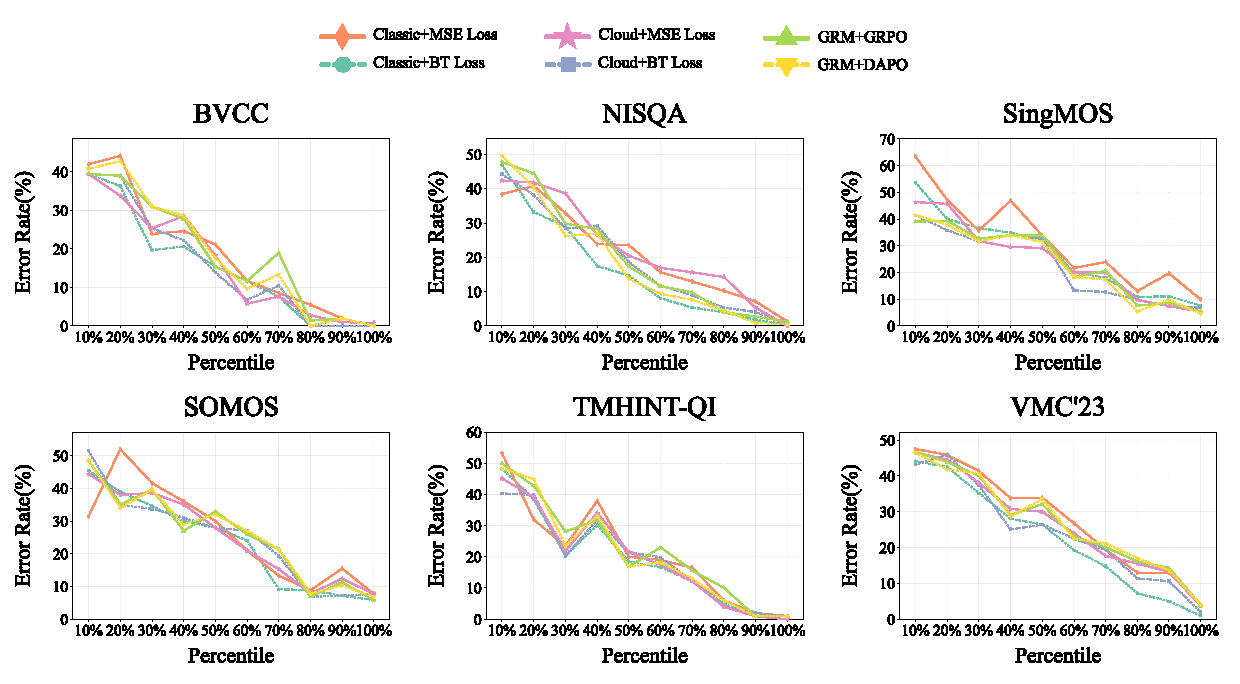
\includegraphics[width=\textwidth]{pictures/error_analysis.pdf}
\end{center}
\caption{Percentile-based error analysis across datasets: error rates are highest for pairs with small MOS differences and decline markedly as the MOS gap widens.}
\label{fig:error-analysis}
\vskip -0.05in
\end{figure}



\subsection{MOS-aware GRM}
\textbf{Design of the MOS-aware reward function.}
GRMs offer a flexible and interpretable framework for reward modeling, allowing the reward signal to be decomposed and extended. During the original GRM reinforcement learning process, the Accuracy reward considers only whether the model correctly ranks the quality of an audio pair, treating all pairs as equally informative. This uniform treatment overlooks the inherent difficulty of pairs with small MOS differences, which may constrain the model’s ability to learn fine-grained quality distinctions. To address this limitation, we introduce the MOS-difference reward, which explicitly incorporates the MOS gap of each audio pair into the reward function:

\begin{equation}
\text{MOS-difference reward}=\left\{
                \begin{array}{lcl}
                        0.5*(1.0+cos(\Delta MOS*\pi))  &     & if\ \ S(c)>S(r),\\
             0.5*(-1.0+cos(\Delta MOS*\pi))  &     & otherwise\\
                \end{array} \right.
\end{equation}

Specifically, $\Delta MOS$ is obtained by normalizing the original MOS gap by the 90th percentile of MOS differences in the dataset and clamping the resulting value to the [0,1] range to mitigate the influence of extreme outliers. Based on the Accuracy reward and the MOS-difference reward, the final MOS-aware reward is defined as follows:

\begin{equation}
\text{MOS-aware reward}=\text{Accuracy reward}+\text{MOS-difference reward}.
\end{equation}

This formulation offers two key advantages. First, it enables adaptive scaling of the reward based on the relative difficulty of each sample pair: for pairs with small MOS differences, correct predictions are assigned a relatively larger reward while incorrect predictions incur a relatively smaller penalty; for pairs with large MOS differences, the reward and penalty are modulated accordingly.
Second, the cosine-based shaping ensures smooth transitions at both ends of the scale. By adjusting the reward according to the implied difficulty, the MOS-aware design provides a more informative learning signal, encouraging the model to attend to subtle perceptual distinctions while still penalizing clearly incorrect predictions.

\definecolor{tealblue}{RGB}{0,180,140}


\begin{table}[t]
\centering
\setlength{\belowcaptionskip}{0.2cm}

\caption{Evaluation results of MOS-aware GRMs with GRPO and DAPO on MOS-RMBench. 
Numbers in \textcolor{tealblue}{parentheses} denote absolute improvements over baseline GRM.}
\label{tab:MOS-aware-GRM}
\renewcommand{\arraystretch}{1.1} % 行距

\resizebox{\textwidth}{!}{
\begin{tabular}{lccccccc}
\toprule
\textbf{Models} & \textbf{BVCC} & \textbf{NISQA} & \textbf{SingMOS} & \textbf{SOMOS} & \textbf{TMHINT-QI} & \textbf{VMC'23} & \textbf{Overall} \\
\midrule
MOS-aware GRM+GRPO &
83.10 \textcolor{tealblue}{(+0.60)} &
81.47 \textcolor{tealblue}{(+1.16)} &
76.50 \textcolor{tealblue}{(+0.10)} &
75.80 \textcolor{tealblue}{(+1.20)} &
80.40 \textcolor{tealblue}{(+2.30)} &
74.13 \textcolor{tealblue}{(+1.00)} &
78.00 \textcolor{tealblue}{(+1.06)} \\
MOS-aware GRM+DAPO &
83.40 \textcolor{tealblue}{(+0.80)} &
82.14 \textcolor{tealblue}{(+0.09)} &
78.40 \textcolor{tealblue}{(+0.90)} &
75.10 \textcolor{tealblue}{(+0.70)} &
79.90 \textcolor{tealblue}{(+0.60)} &
73.57 \textcolor{tealblue}{(+0.44)} &
78.08 \textcolor{tealblue}{(+0.48)} \\
\bottomrule
\end{tabular}
}
\end{table}



\begin{figure}[htbp]
\setlength{\abovecaptionskip}{-1pt}
  \centering
  \begin{subfigure}{0.48\textwidth}
    \centering
    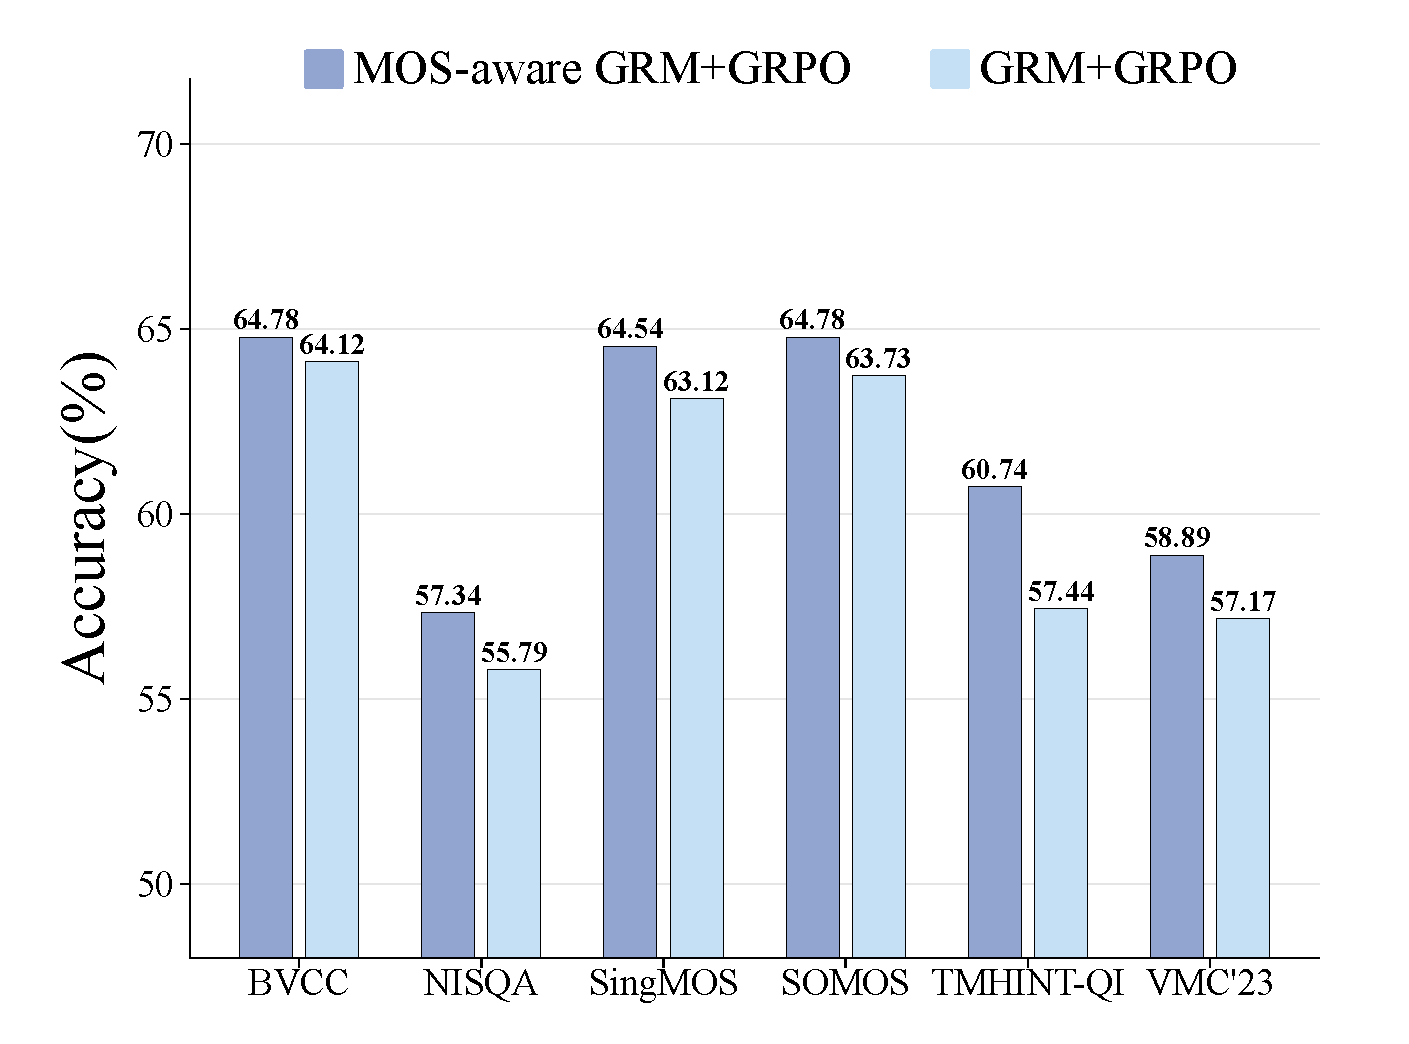
\includegraphics[width=\linewidth]{pictures/MOS-aware-GRM-GRPO.pdf}
    \caption{Training strategy: GRPO}
    \label{fig:grpo}
  \end{subfigure}
  \hfill
  \begin{subfigure}{0.48\textwidth}
    \centering
    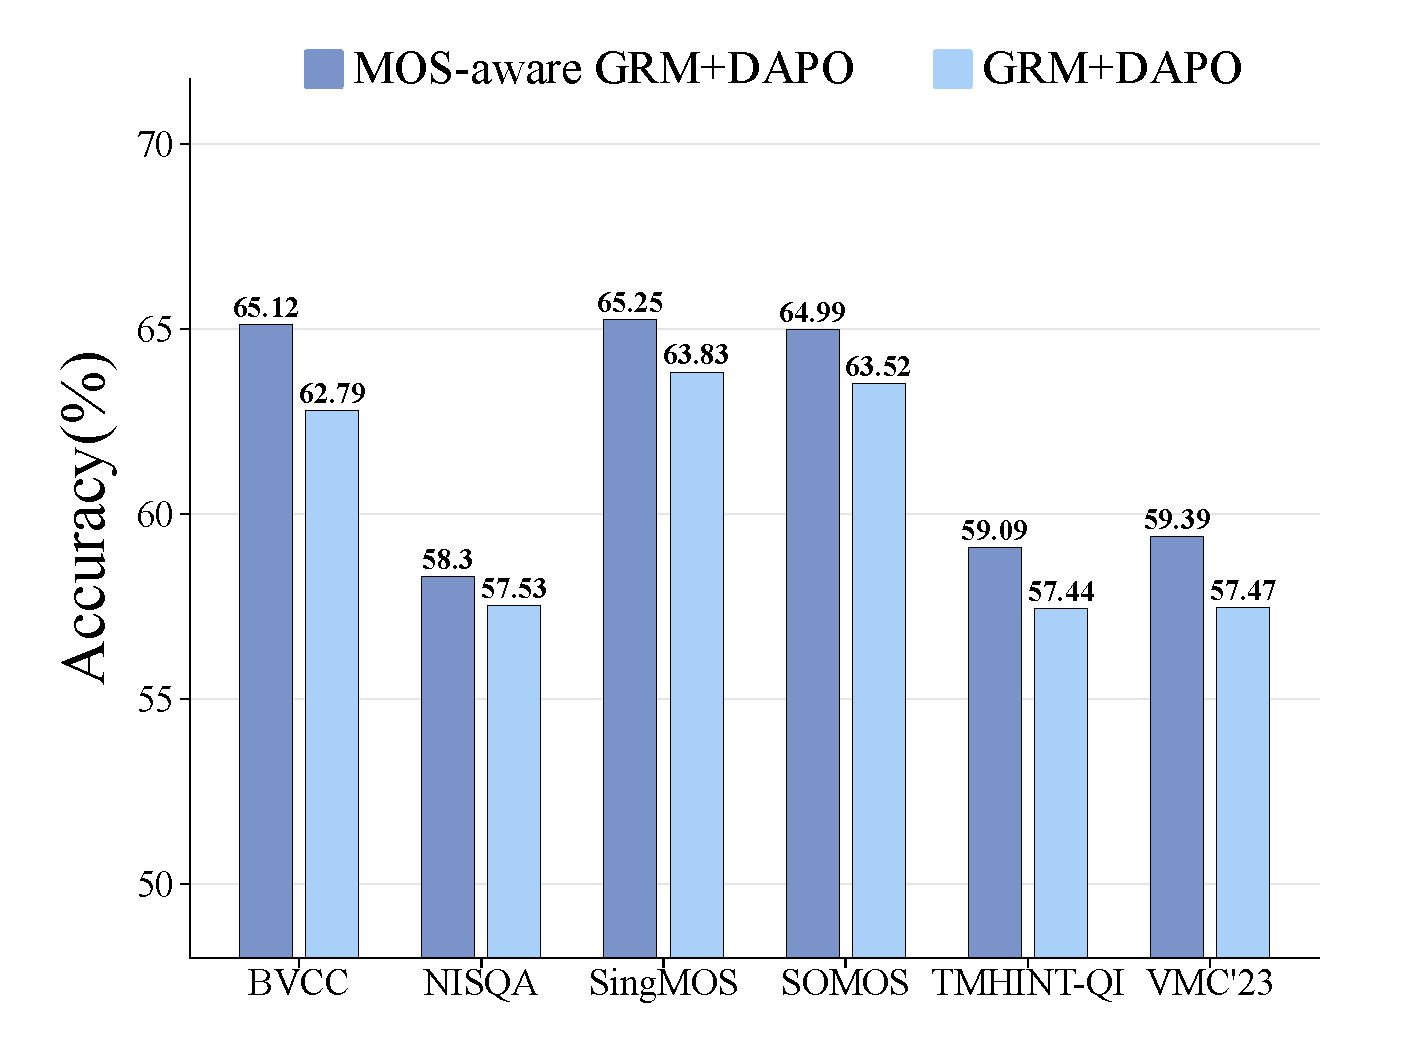
\includegraphics[width=\linewidth]{pictures/MOS-aware-GRM-DAPO.pdf}
    \caption{Training strategy: DAPO}
    \label{fig:dapo}
  \end{subfigure}
  \vspace{2mm}
  \caption{Performance comparison of MOS-aware GRMs and standard GRMs trained with different reinforcement methods on samples with MOS difference $\le 0.5$.}
  \label{fig:MOS-aware-GRM}
\vskip -0.05in
\end{figure}


\textbf{Impact of MOS-aware reward on GRM performance.}
To evaluate the effectiveness of the proposed MOS-aware reward, we incorporate it into the GRM training process under both GRPO and DAPO strategies, while keeping all other training configurations unchanged. This design enables a direct comparison with baseline GRM models that rely solely on the Accuracy reward.
Table~\ref{tab:MOS-aware-GRM} summarizes the overall results, showing that MOS-aware GRMs achieve consistent improvements over their baseline counterparts across all evaluation scenarios.


To further examine performance on perceptually challenging pairs, we evaluate models  on sample pairs with a MOS difference threshold of 0.5.  Figure~\ref{fig:MOS-aware-GRM} presents the corresponding results. Across all datasets, MOS-aware GRMs consistently outperform the baselines on these fine-grained comparisons. For illustration, with the GRPO strategy, accuracy increases from 57.44\% to 60.74\% on THMINT-QI and from 57.17\% to 58.89\% on the OOD VMC'23 dataset; under the DAPO strategy accuracy improves from 62.79\% to 65.12\% on BVCC and from 57.47\% to 59.39\% on VMC'23. 
These results demonstrate that incorporating MOS difference information into the reward function produces stable and statistically significant gains. The MOS-aware design provides a more informative, difficulty-sensitive learning signal that strengthens GRM's capacity to capture fine-grained perceptual quality differences beyond what the conventional Accuracy reward achieves.